\documentclass[letterpaper]{article}
\usepackage{amsmath}
\usepackage{algorithm}
\usepackage{multirow}
\usepackage{graphicx}

\DeclareMathOperator*{\argmin}{arg\,min}

\begin{document}
\title{ECON 199 Final Exam}
\author{Will Koster}
\date{May 14, 2020}
\maketitle

\clearpage

\section{Problem 1}
Starting in season 3, episode 4 and going through the end of the season, the HBO series \textit{The Wire} showed a novel policing strategy referred to on the street as ``Hamsterdam.'' Bunny Colvin, the head of the police department in the Western district of Baltimore, found an area of the district with very nearly no residents at all and explained to the middle management of the local drug gang that they could go about their business unmolested by the police so long as it was conducted in this area. \\
In game theoretic terms, interactions between drug gangs and police can be partially modeled as a two-player, sequential game that is constantly being played. The police always play first, and they have the option to either allow drugs nowhere, or effectively allow them in some locations and not others. If the police enforce drug laws everywhere, the gangs can either stop selling or sell wherever they please. \\
If the police selectively enforce drug laws, the gangs can stop selling, sell wherever they want, or sell where the police allow them to. If the drug gangs stop selling, the police have a huge utility gain\footnote{An argument could be made that the drug market is a nontrivial employer in some locales, and putting hundreds or thousands of people in community out of work could certainly cause other problems to appear, but its very likely that the police will still end up better than they were before.}, but the drug dealers are now unemployed. \\
If they keep selling even as the police enforce the laws, they can continue to have income, but the fact that the police keep harassing them means that their overhead is substantial. The police have to contend with the murders and drug addicts that are fueled by the drug market. \\
If the police only selectively enforce the laws and the drug gangs keep selling where the police allow them, the drug gangs lose little revenue compared to selling everywhere, since demand for drugs is relatively inelastic in the short- to medium-term, but have much lower overhead. The police still have to deal with the social problems caused by drug addiction, but they can limit murders (which are often a tool to prevent informing the authorities) and provide social services (eg in the show, aid workers come to Hamsterdam to do AIDS testing and distribute condoms). If the drug gangs continue selling wherever they want, the outcome is the same as what would happen if laws were enforced everywhere, since uninhabited areas are not competitive from a business perspective. \\

Based on this, we can make a game tree for this game. The rollback equilibrium (where the police allow drug sales in a defined area and the gangs abide by it) is highlighted in lime green. \\
\hspace*{-1.5in}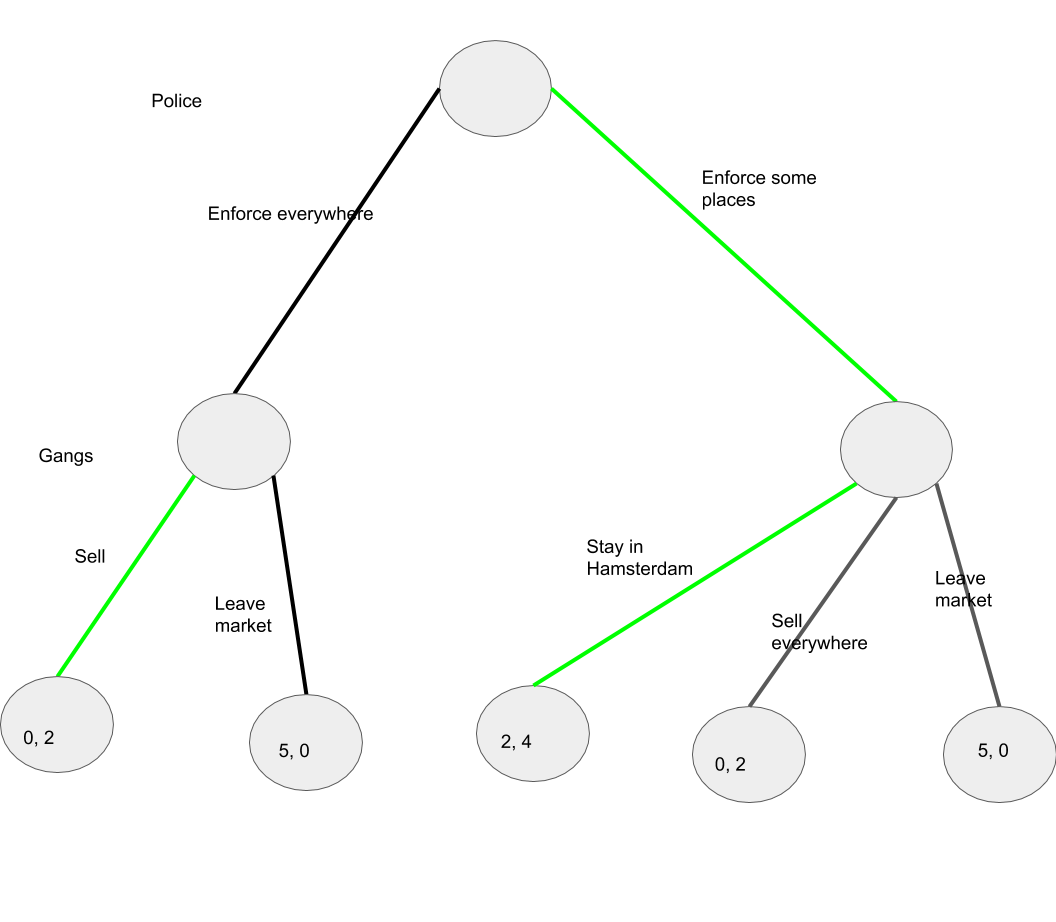
\includegraphics[scale=0.7]{fig1} \\
I'm not familiar with an paradigm games that match this format. \\
The police, after Colvin's epiphany, make drugs effectively legal, and the drug gangs, after some initial trepidation, move all their business into these legal zones. Therefore, both sides act rationally in the show.
\section{Problem 2}
The question all the cool kids are asking these days is whether to wear a mask when you go outside. If you wear one, you will protect other people from any illness you may have, but you won't protect yourself very much and you'll be uncomfortable. If you don't wear one, you'll put other people in some danger but you'll be more comfortable. Therefore, if everyone except you wears a mask, you are both protected and comfortable, and if you alone wear a mask, you're both unprotected and uncomfortable. We can model this as a 2-player simultaneous game with the payoff matrix below. \\
    \begin{tabular}{|c|c|c|c|}
        \hline
        & \multicolumn{3}{c|}{Player B}       \\ \hline
        \multirow{3}{*}{Player A} & & Mask & No Mask \\ \cline{2-4}
        & Mask  & 2, 2  & 0, 3    \\ \cline{2-4}
        & \multicolumn{1}{c|}{No Mask} & \multicolumn{1}{c|}{3, 0} & 1, 1    \\ \hline
    \end{tabular} \\
    The Nash Equilibrium is (No Mask, No Mask). This is a classical Prisoner's Dilemma, and yet we've (by now) all seen people wearing masks outside even though the optimal strategy is to leave your mask at home. This is probably because the payoff matrix does not account for social pressure, which is hard to quantify but clearly affects people's actions. These social pressures vary based on location, and in places where they are low, game theory can yield the strategically optimal action, but in places with stronger social pressure, observation suggests that this formulation of the game does not include all incentives.
\section{Problem 3}
Collude

\end{document}
